\addbibresource{reference.bib}

\chapter{Atlas TPX}\label{atlas}
Atlas TPX je síť 15\footnote{V průběhu LS3\textsuperscript{\ref{ls}} (plánováno 2017 - 2018) je plánováno rozšíření teto sítě o nové detektory} hybridních pixelových detektorů typu Timepix \ref{det:tim}, nainstalovaných na různé pozice experimentu Atlas na LHC\footnote{z angl. Large Hadron Collider} v CERN během LS2\footnote{\label{ls}z angl. long shutdown - dlouhodobá technologická přestávka LHC} (leden 2013 až březen 2015) je následníkem svého předchůdce - sítě Atlas MPX (viz \ref{atlas:mpx}). Hlavní motivací výměny této sítě bylo využití nových technologií, především pak nového detekčního čipu Timepix. Ten na rozdíl od svého předchůdce Medipix2 \ref{det:med} umožňuje rozšíření naměřené informace i o časovou oblast (viz \ref{det:tim}). To nově umožňuje provozovat detektory v módech TOA\footnote{z angl. Time of Arrival - čas příletu částice v hodinových cyklech detektoru od začátku akvizice} a TOT\footnote{z angl. Time Over Treshold - počet hodinových cyklů, kdy komparační napětí je větší, než referenční (ekvivalent energie deponované částice, viz kapitola \ref{calib})}. 

Další změnou oproti svému předchůdci je, že každý detektor obsahuje dva detekční čipy s tloušťkami $300~\mu m$ a $500~\mu m$, umístěné předními stranami k sobě - viz \ref{fig:tpx_detector_layers}. To přináší možnost měřit koincidence. Když částice projde oběma vrstvami  detektoru a zároveň v každé nechá jisté měřitelné množství své energie, je detekována oběma vrstvami a je možné zpětně zrekonstruovat její trajektorii. Tyto koincidence se nejsnáze detekují, pokud oba Timepix čipy pracují v módu TOA - jelikož rychlost částic se blíží rychlosti světla, je vysoce pravděpodobné, že zasažené pixely budou mít stejnou hodnotu.


\begin{figure}[th]
	\begin{center}
		\begin{subfigure}{6cm}
			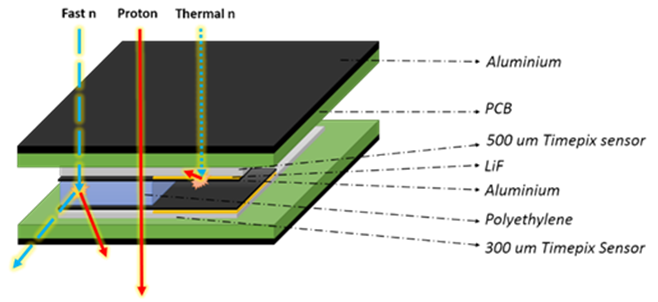
\includegraphics[width=6cm]{figures/tpx_lay.png}	
			\caption{Vrstvy detektoru}
			\label{fig:tpx_detector_layers}
		\end{subfigure}
		\hspace{0.5cm}
		\begin{subfigure}{5cm}
			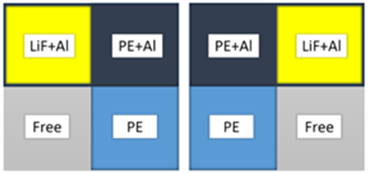
\includegraphics[width=5cm]{figures/tpx_conv.png}
			\caption{Rozmístění konvetorů}
			\label{fig:tpx_detector_convertors}
		\end{subfigure}
		\caption{Atlas TPX detektor - vrstvy a rozmístění konvertorů}
		\label{fig:tpx_detector}
	\end{center}			
\end{figure}

Mezi vrstvami detektoru je umístěn konvertující materiál pro detekci termálních a rychlých neutronů. Rozmístění těchto konvertorů je na obrázku \ref{fig:tpx_detector_convertors}.

Hlavním úkolem Atlas TPX je online monitorování spektrální charakteristiky velice různorodého radiačního prostředí Atlas experimentu, založeny na prostorovém uspořádání sítě a (vzhledem k aktuálním módu detektoru) i informaci o deponované energii zainteragovaných částic a časovou informaci. 


Detektory, instalované blízko interakčnímu bodu, jsou rovněž použity jako monitory integrované luminozity, což je veličina, která udává počet realizovaných srážek, resp. s intenzitou svazku urychlovače. Ve \cite{wagner:o_lhc} se uvádí, že je to veličina, která v případě srážení dvou proti sobě letících svazků ukazuje, jaký je součin počtů částic v jednotlivých svazcích prolétajících jednotkovou plochou v srážkové oblasti, vynásobený počtem obletů svazků za jednotku času (nejčastěji se vyjadřuje v jednotkách na centimetr čtvereční a sekundu).

%********************************************************************************
% Atlas MPX
%********************************************************************************
\section{Atlas MPX}\label{atlas:mpx}
Atlas MPX\cite{Vykydal200935}\cite{atlasmpx} je předchůdcem detektorové sítě Atlas TPX, která v současné době je plně nahrazena. Skládala se z 16 Medipix2 detektorů, které byly instalovány na různé pozice Atlas detektoru - viz obr. \ref{fig:mpx_positions}. Hlavním cílem této sítě bylo měření vlastností radiačního pole uvnitř experimentu Atlas, jeho složení, spektroskopických charakteristik a částečně také přispěla k měření neutronů. 

\begin{figure}[ht]
	\begin{center}
		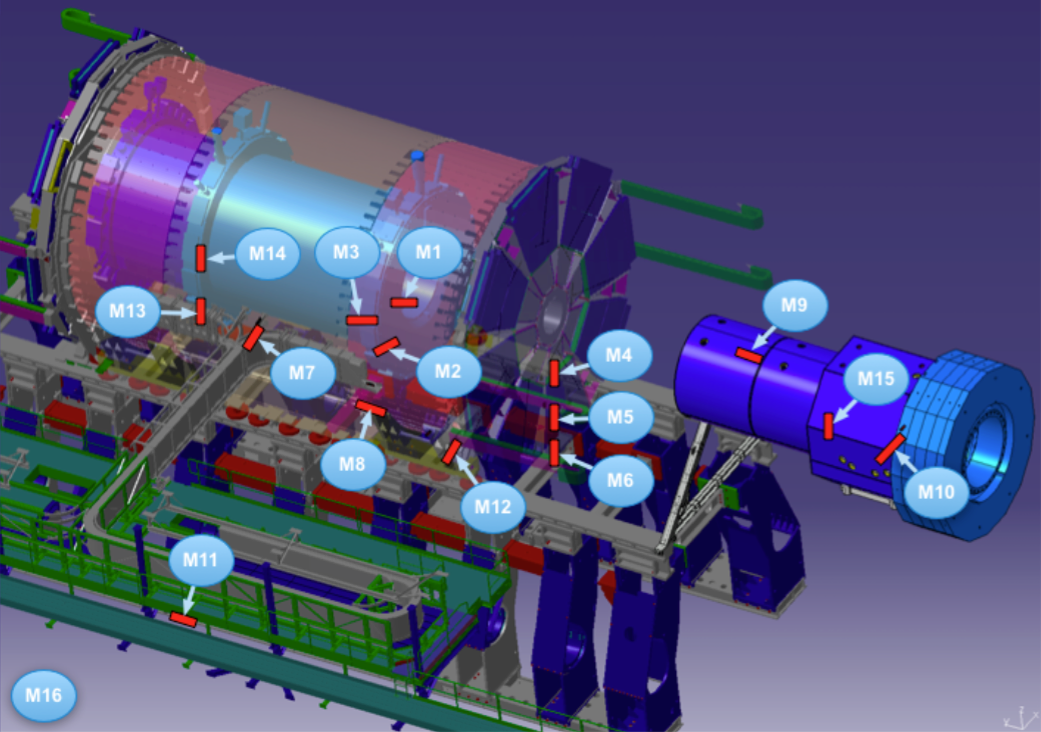
\includegraphics[width=11cm]{figures/mpx_positions.png}
		\caption{Atlas MPX s přehledem rozmístění detektorů}
		\label{fig:mpx_positions}
	\end{center}
\end{figure}

Všechny detektory operovaly v tzv. \texttt{Medipix módu}, který se vyznačují tím, že v rámci jedné akvizice počítá počet částic, které interagovaly pixelovou maticí detektoru a jejichž deponovaná energie byla vyšší, než prahová. Na obrázku \ref{fig:mpx_cluster} je znázorněn snímek z jednoho detektoru s detailem zachycených částic. Na obrázku vpravo nahoře je částice typu \texttt{heavy blob} (těžce nabitá částice, jejíž trajektorie byla kolmá s povrchem detektoru), vpravo dole je pak zachycena částice typu \texttt{heavy track} (také těžce nabitá částice, která ale přiletěla pod větším a proto zanechala větší stopu) - více klasifikaci částic se dočtete v podkapitole \ref{det:ca}.


\begin{figure}[ht]
	\begin{center}
		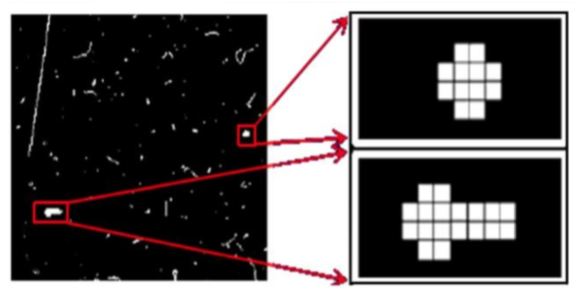
\includegraphics[width=7cm]{figures/mpx_cluster.png}
		\caption{Snímek z Atlas MPX detektoru s výřezem zachycených částic (převzato z \cite{atlasmpx})}
		\label{fig:mpx_cluster}
	\end{center}
\end{figure}


Každý z těchto detektorů byl osazen $300~\mu m$ tlustým křemíkovým senzorem, který byl pokryt konvertory pro lepší detekční účinnost neutronů (obr. \ref{fig:mpx_lay}).

\begin{figure}[ht]
	\begin{center}
		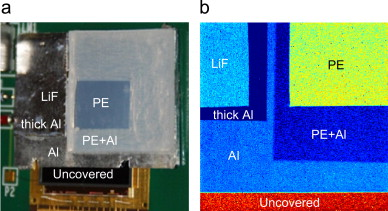
\includegraphics[width=7cm]{figures/mpx-layers.jpg}
		\caption{Fotografie znázorňující Medipix2 detektor s neutronovými konvertory (převzato z \cite{Vykydal200935})}
		\label{fig:mpx_lay}
	\end{center}
\end{figure}

\subsection{Hardwarová a softwarová architektura sítě Atlas MPX}
Tato síť se skládala z 16 \texttt{Medipix2} \ref{det:med} detektorů, které byly pomocí USB vyčítacího rozhraní \texttt{FITPix} \ref{det:fitpix} připojeny ke třem počítačům (z důvodu distribuce toku dat a výkonu). Na každém počítači se o komunikaci s detektory staral software \texttt{Pixelman} \ref{det:pixelman}, který řídil akvizici dat, nastavování parametrů detektorů apod. 

Pro vzdálené obládání každého byl vyvinut plugin pro Pixelman, který umožňoval jeho rozšíření o TCP/IP ovládací vrstvu. Pomocí jednoduchého textového protokolu bylo tedy možné řídit každý ze třech uzlů. Pro tyto účely byla vyvinuta centrální řídící aplikace \cite{Turecek2011S45}, pomocí které bylo možné řídit řídit akvizici všech detektorů a nastavovat jejich parametry. Tato aplikace poskytovala webové rozhraní (obr. \ref{fig:mpx_web}), které díky tou dobou méně striktní CERNské politiky síťové bezpečnosti bylo možné tento experiment ovládat z internetu.

\begin{figure}[ht]
	\begin{center}
		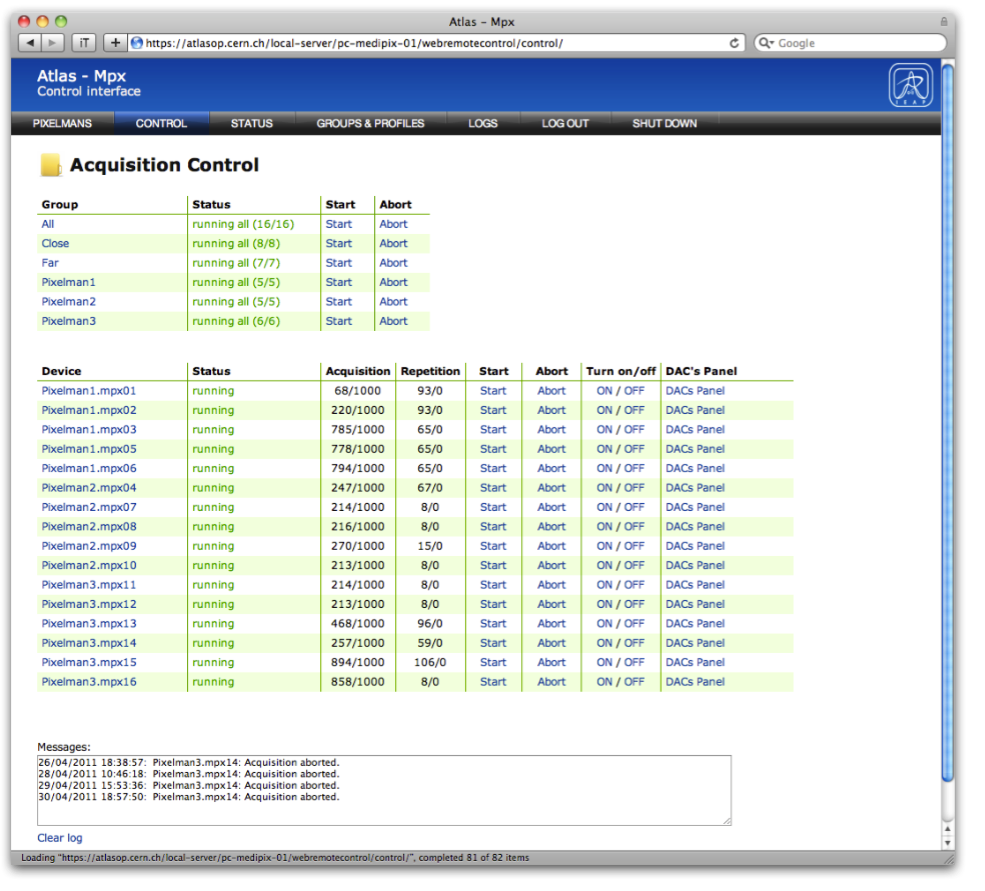
\includegraphics[width=10cm]{figures/mpx_web.png}
		\caption{Atlas MPX - řídící aplikace (převzato z \cite{TurecekThesis2011})}
		\label{fig:mpx_web}
	\end{center}
\end{figure}

%********************************************************************************
% Hardwarová architektura
%********************************************************************************
\section{Hardwarová architektura}\label{atlas:hw_arch}
Při návrhu hardwarové architekty sítě Atlas TPX musela být zohledněna zvýšená intenzita radiačního a elektromagnetického pole v okolí Atlas detektoru. Snahou proto bylo, co nejvíce hardwarových komponent umístit z dosahu tohoto pole. Z pohledu hardwarové instalace naší detektorové sítě se prostory Atlas experimentu dělí na dvě části - \texttt{UX15} a \texttt{USA15} (viz obr. \ref{fig:tpx_hw_diagram}). V \texttt{UX15} se nachází vlastní experiment. V tomto prostoru byly umístěny jen vlastní detektory (na obr. \ref{fig:tpx_hw_diagram} \texttt{TPX01} až \texttt{TPX15}) a zbytek sítě je instalován v \texttt{USA15}, kterou od zbytku experimentu dělí cca $60~m$ tlustá železobetonová stěna. Tady se nachází vyčítací elektronika a další nezbytný hardware.

\begin{figure}[t]
	\begin{center}
		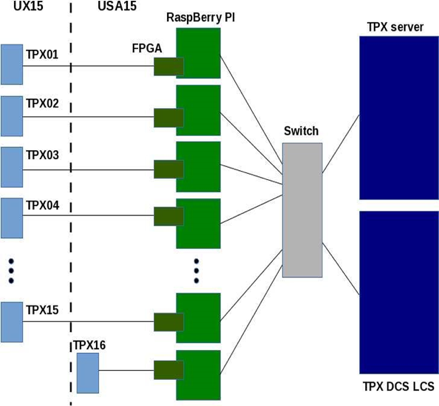
\includegraphics[width=8cm]{figures/tpx_hw_diagram.png}
		\caption{Atlas TPX - diagram hw komponent}
		\label{fig:tpx_hw_diagram}
	\end{center}
\end{figure}

Na obrázku \ref{fig:tpx_hw_foto} je fotografie fotografie těchto komponent. Jak již bylo zmíněno výše, detektor (z obr. \ref{fig:tpx_hw_foto}, na obr. \ref{fig:tpx_hw_diagram} jako \texttt{TPX01} až \texttt{TPX15}) se skládá z dvojice detekčních čipů \texttt{Timepix2}, které jsou pomocí \texttt{LVDS} zesilovačů a cca $100~m$ dlouhých ethernetových kabelů propojeny se zařízením \texttt{AtlasPix} (obr. \ref{fig:tpx_hw_foto} dole), které vzniklo modifikací vyčítacího rozhraní \texttt{FITPix} \ref{det:fitpix}. Toto zařízení obsahuje \texttt{FPGA}\footnote{z angl. Field Programmable Gate Array (programovatelné hradlové pole)}, minipočítač \texttt{Raspberry Pi} a další podpůrnou elektroniku. 

\texttt{FPGA} se stará o komunikaci s \texttt{Timepix2} detektory, v rámci které dochází k nastavování řídících registrů \texttt{Timepix2} čipů, ovládání akvizice, vyčítání dat, řízení triggeru\footnote{řídící signál, který spouští resp. zastavuje (dle konfigurace) akvizici detektoru} apod.

\begin{figure}[t]
	\begin{center}
		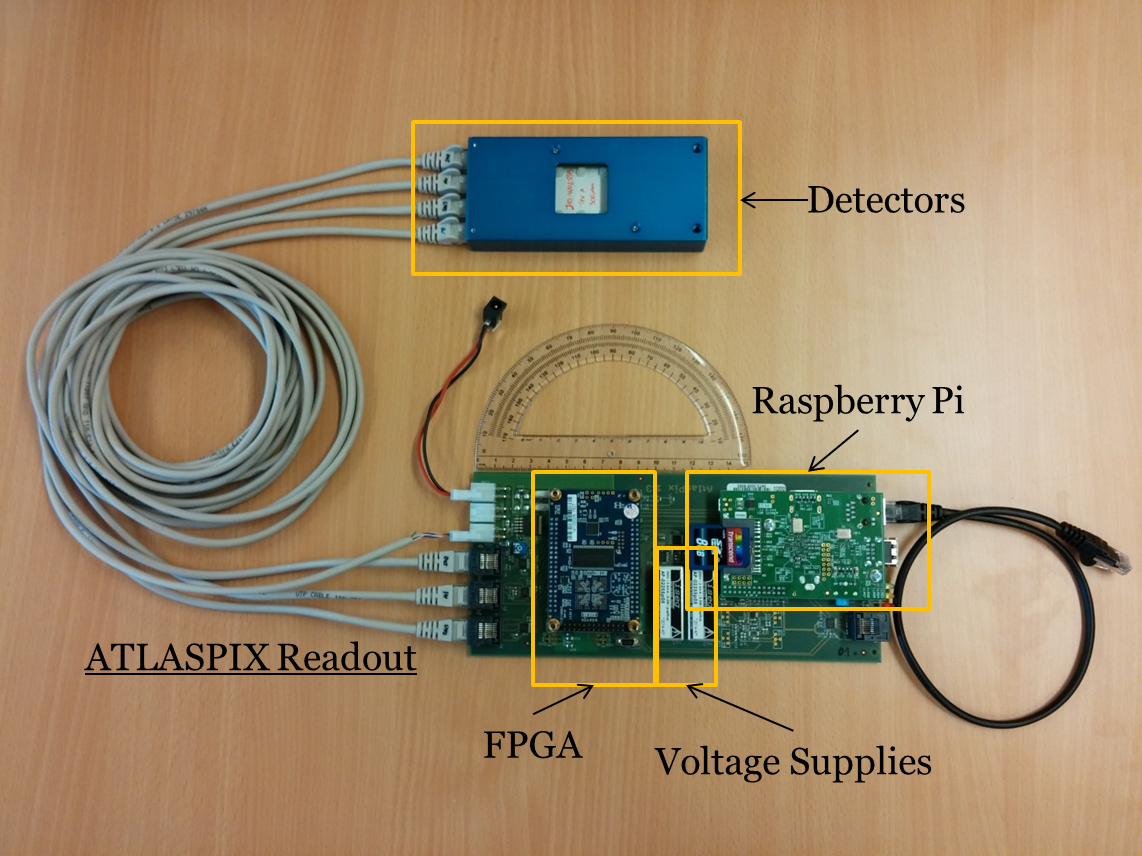
\includegraphics[width=8cm]{figures/tpx_hw_foto.png}
		\caption{Atlas TPX - fotografie hw komponent}
		\label{fig:tpx_hw_foto}
	\end{center}
\end{figure}

Dalším článkem tohoto řetězce je minipočítač \texttt{Raspberry Pi}, který plní dvě úlohy. Tou první je komunikace s \texttt{FPGA} pomocí \texttt{SPI}\footnote{z angl. Serial Peripheral Interface (sériové periferní rozhraní)} rozhraní, deserializace (získání dat ze struktury komunikačního protokolu) a derandomizace (není zaručena časová posloupnost) surových dat z \texttt{FPGA}. Druhou úlohou tohoto zařízení je poskytování API\footnote{z angl. Application Programming Interface (aplikační programovací rozhraním)} vyšším řídícím vrstvám této sítě pomocí specifikovaného komunikačního protokolu a klasického ethernetového rozhraní.

Všechny tyto zařízení jsou pomocí ethernetového switche propojeny s \texttt{TPX serverem}, který je centrálním bodem této sítě, který jí pomocí řídícího softwaru \ref{atlas:cont} a komunikačního protokolu \ref{atlas:cont:det} ovládá. Zároveň je k síti připojen i \texttt{TPX DCS\footnote{z angl. Data Control System} server}, pomocí kterého jsou různé stavové informace \texttt{Atlas TPX} sítě předávány CERNu, resp. Atlas experimentu. Tyto stavové informace jsou převážně hardwarového charakteru (na př. napětí, časování apod.), ale také jsou předávána data o počtu pořízených snímků, jejich okupanci apod.




\clearpage
\section{Softwarová architektura}\label{atlas:sw_arch}
\section{Řídící software}\label{atlas:cont}
\subsection{Řízení detektorů}\label{atlas:cont:det}
\subsection{REST API server}
\subsection{Zpracování a ukládání dat}


